\section{Module M6}

\note{votre lecteur ne connait pas votre démarche ni
pourquoi un tel résultat démontre le bon fonctionnement – vous devez l'expliquez brièvement.}

\note{Nous ne consulterons pas le dépôt de vos fichiers Xilinx (sauf
dans des cas particuliers) ce qui signifie que votre rapport doit être complet en lui-même.}

\quicktable{Plan de vérification du module M6 -- Calcul de puissance}{mef-m6}{p{4cm}p{5cm}p{6cm}l}{
  \toprule
  \textbf{Objectif Ciblé} &
  & \multirow{2}{*}{\textbf{Valider la MEF calcul de puissance d'ondes}}
  & \\
  Condition à proscrire
  & Ondes ayant une fréquence plus haute que \SI{24}{\kilo\hertz}
  &
  & \\
  \midrule
  \textbf{Test}
  & \textbf{Action}
  & \textbf{Résultat attendus}
  & \cboxtick \\
  \midrule
  Condition initial
  & Mettre les interrupteurs à 0010 et une onde sans amplitude
  & La puissance en sortie reste à 0.
  & \cbox\\
  Reset initial
  & \texttt{BTN3} à 1 et onde sans amplitude.
  & La valeur de la puissance devient 0 et reste à 0 après.
  & \cbox\\
  Test d'une onde sinuosïdale
  & Mettre une onde sinus de \SI{1}{\kilo\hertz}. À amplitude maximum
  & La puissance augmente et oscille en suivant l'amplitude du signal d'entrée
  & \cbox\\
  Test d'une onde sinusoïdale avec bruit
  & Mettre une onde sinus de \SI{1}{\kilo\hertz} avec un peu de bruit. À amplitude maximum
  & La puissance augmente et oscille a la même fréquence que le signal d'entrée. Observation d'atténuation du bruit.
  & \cbox\\
  Test d'une onde Carré
  & Mettre une onde carré de \SI{1}{\kilo\hertz} à amplitude maximum
  & La puissance augmente vers le maximum et reste stable.
  & \cbox\\
  Test de haute fréquences
  & Mettre une onde sinus de \SI{20}{\kilo\hertz}
  & La puissance oscille en fonction de l'amplitude du signal. la valeur de la puissance reste en moyenne plus haute que l'onde de \SI{1000}{\hertz} (à cause de l'accumulation).
  & \cbox\\
  Test de saturation
  & Un signal d'amplitude maximum envoyé en continue
  & La puissance atteint le maximum après quelques échantillons et aucun débordement se produit.
  & \cbox\\
  Test d'amplitude fix basse
  & Onde carrée d'amplitude 0.5 à -0.5 envoyé en entrée
  & la puissance atteint la moitié du maximum après quelques échantillons et reste stable
  & \cbox\\
  \bottomrule
}

\begin{figure}[H]
  \centering
  \begin{subfigure}{.496\linewidth}
    \centering
    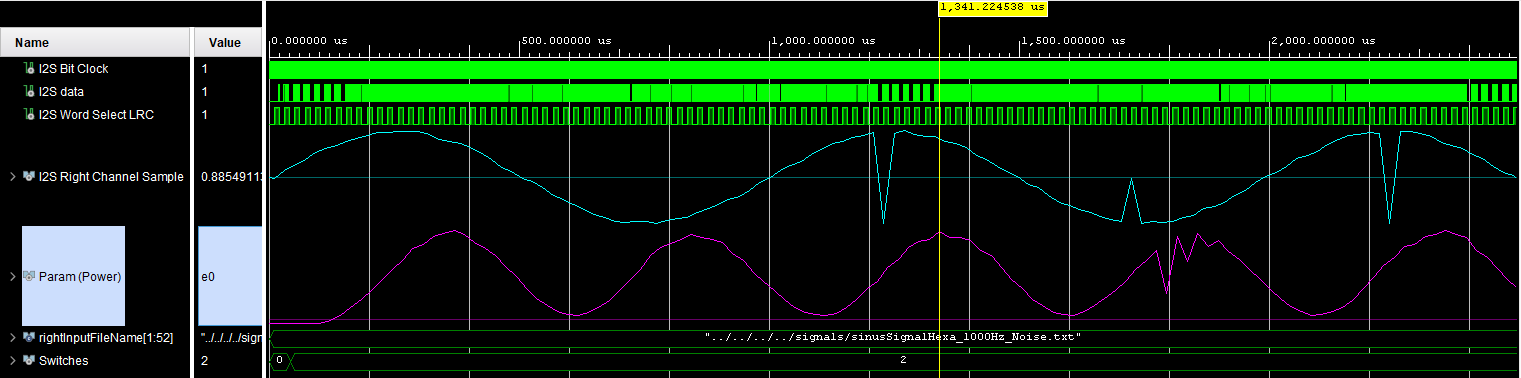
\includegraphics[width=\textwidth]{assets/chrono-m6-1000hz-sin-noisy.png}
    \caption{Signal sinusoïdal bruité à \SI{1}{\kilo\hertz}}
    \label{fig:chrono-m6-1000hz-sin-noisy}
  \end{subfigure}
  \begin{subfigure}{.496\linewidth}
    \centering
    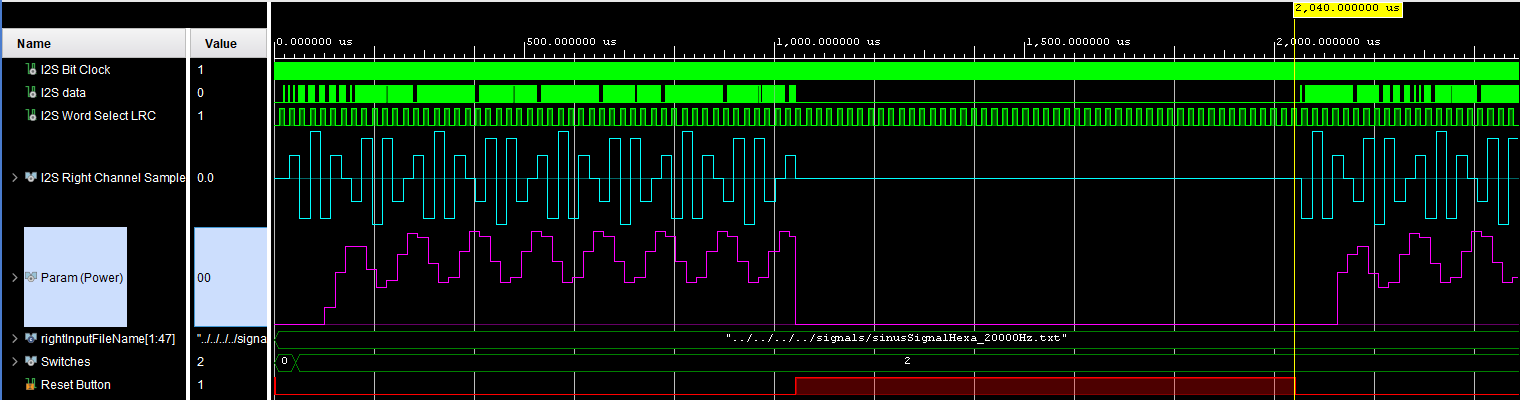
\includegraphics[width=\textwidth]{assets/chrono-m6-reset-and-20000hz.png}
    \caption{Post-réinitialisation et signal à \SI{20}{\kilo\hertz}}
    \label{fig:chrono-m6-reset-and-20000hz}
  \end{subfigure}
  \begin{subfigure}{.496\linewidth}
    \centering
    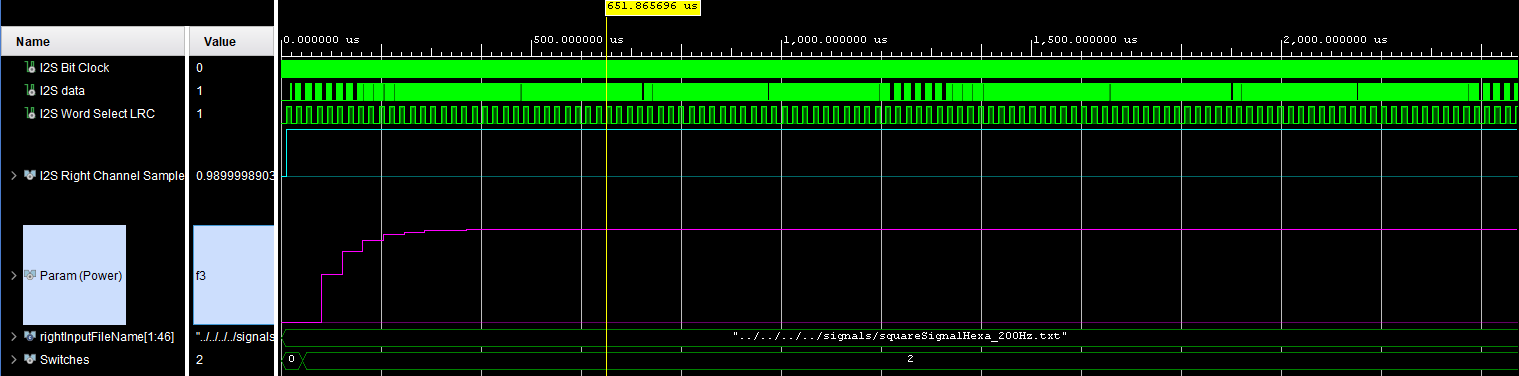
\includegraphics[width=\textwidth]{assets/chrono-m6-saturation-works.png}
    \caption{Saturation du module}
    \label{fig:chrono-m6-saturation-works}
  \end{subfigure}
  \begin{subfigure}{.496\linewidth}
    \centering
    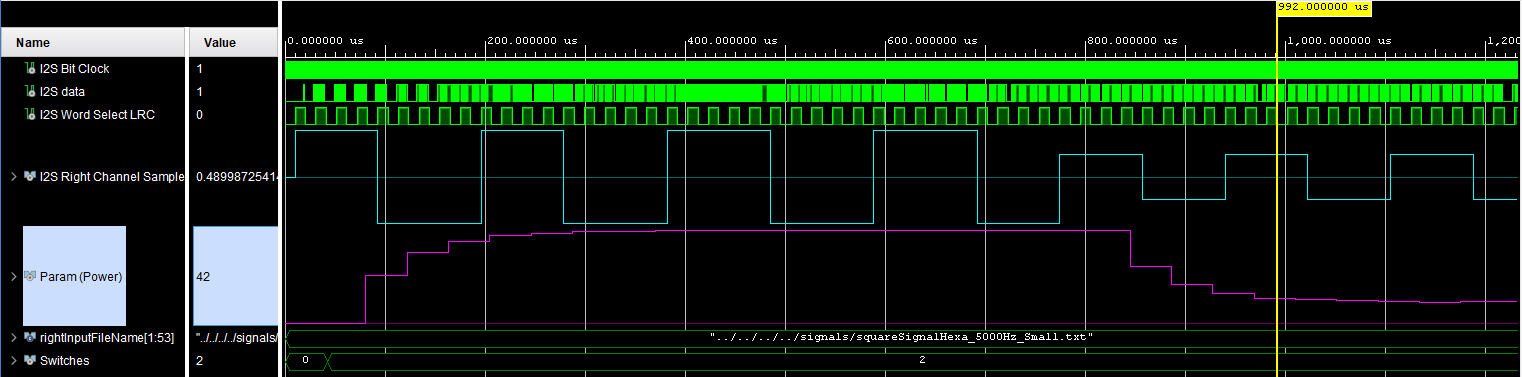
\includegraphics[width=\textwidth]{assets/chrono-m6-square-5000hz-2in1.png}
    \caption{Signal carré à 5000 Hz avec deux canaux}
    \label{fig:chrono-m6-square-5000hz-2in1}
  \end{subfigure}
  \caption{Chronographes du module M6 sous différentes conditions}
\end{figure}

% \quickfigure{Machine à états finis du module M6}{mef-m6}{}{assets/m6-mef-mermaid.pdf}

\todo{Schéma-bloc du système}

\subsection{Description du fonctionnement}

Le module M6 effectue une estimation de la puissance du signal audio en
appliquant un filtrage exponentiel à moyenne glissante sur les échantillons
entrants. Le calcul s'effectue à chaque front montant de l'horloge
\verb|i_bclk|, lorsque le signal \verb|i_en| est à 1. \\

À chaque activation, la puissance instantanée est calculée en élevant au
carré l'échantillon courant \verb|i_ech|. Cette nouvelle valeur est ensuite
ajoutée à l'historique de puissance, qui est préalablement réduite par un
facteur d'oubli de 31/32. Ce facteur assure que les résultats récents ont
plus de poids que les anciens, tout en limitant la croissance de la valeur
accumulée afin d'éviter un débordement (\emph{overflow}). \\

Le résultat final est stocké dans le registre \verb|oldest_power|. Pour
simplifier l'affichage ou l'utilisation de cette puissance, seuls les bits de
poids fort (\verb|oldest_power(46 downto 39)|) sont extraits et envoyés sur
la sortie \verb|o_param|. \\

Le fonctionnement réponds plus ou moins aux spécifications. 
À cause de la méthode utilisé, la mesure de la puissance ne se stabilise pas assez lentement pour donner un nombre fixes 
à des basses fréquences (chronogramme A \ref{fig:chrono-m6-1000hz-sin-noisy}). Cependant ce chronogramme démontre la résistance au bruit. 
La figure \ref{fig:chrono-m6-reset-and-20000hz} démontre le bon fonctionnement du reset (le tout reste à zéro jusqu’à la relâche du signal en rouge). 
La figure \ref{fig:chrono-m6-saturation-works} démontre que le calcul monte tranquillement vers le maximum (prouvant l'utilisation d'accumulation)
et n'éprouve aucun dépassement restant stable. la figure \ref{fig:chrono-m6-square-5000hz-2in1} démontre que la puissance reste stable et s'adapte 
aux changements d'amplitude du signal entrant dans le module. le chronogramme \ref{fig:chrono-m6-reset-and-20000hz} à une sinus à l'entrée, mais le graphique
à été réalisé avec la fonction d'affichage « hold » se qui donne l'impression d'une onde carré. Les spécification sont 
donc atteinte car un facteur de 31/32 est utilisée et une accumulation en continue est présente. Cependant, l'angle d'approche
serait à revoir afin d'avoir des lectures stables avec des ondes sinusoïdales.

% \todo{Description sommaire du fonctionnement}
%\todo{Plan de vérification}

%\todo{Validation via une simulation avec le banc de test fourni. Vous devez démontrer le
%fonctionnement de vos modules au travers de simulations et expliquez en quoi vous
%répondez aux spécifications. Faites bon usage des curseurs, formattage des données et
%agrandissements pour appuyer vos propos.}
